\section[Руководство пользователя]{РУКОВОДСТВО ПОЛЬЗОВАТЕЛЯ}
\label{sec:user_manual}

\subsection{Системные требования}

Для установки и использования приложения должен использоваться 
X86-совместимый компьютер с тактовой частотой процессора не менее 500 МГц,
объемом оперативной памяти не менее 64~МБ под управлением операционных систем
на базе ядра GNU/Linux, *BSD, Windows.

Для успешной сборки приложения на компьютере пользователя должна быть
предварительно установлена утилита GNU Make и компилятор языка C.
Данные программы находятся в репозиториях всех дистрибутивов на базе GNU/Linux,
*BSD, а также доступны в Windows в пакетах программ 
Cygwin и MinGW~\cite{cygwin, mingw}.

\subsection{Установка}

Установка разрабатываемой программы предполагает загрузку исходного текста
программы и компиляцию этого исходного текста.

% Возможны два варианта загрузки исходного кода: в виде архива и 
% в виде репозитория git. Рассмотрим каждый из них.

Для того, чтобы загрузить исходный код в виде архива в операционной системе 
на базе GNU/Linux, достаточно выполнить
команды, представленные на рисунке~\ref{lst:zip_installation}.

\begin{lstlisting}[basicstyle=\scriptsize\ttfamily,
                   numberstyle=\scriptsize\ttfamily,
                   xleftmargin=7mm,
                   language=bash,
                   caption=Команды установки архиватора \\ 
                   без создания репозитория,
                   label=lst:zip_installation]
wget https://github.com/budnyjj/huffman/archive/master.zip
unzip master.zip
cd master
make
\end{lstlisting}

Первая команда загружает архив с исходным кодом с сервиса github.com,
вторая производит распаковку архива с исходным кодом,
третья меняет текущую директорию на директорию с исходным кодом,
четвертая производит сборку приложения.

% Для того, чтобы загрузить исходный код в виде репозитория git в
% операционной системе на базе GNU/Linux, достаточно выполнить
% команды, представленные на рисунке~\ref{lst:git_installation}.

% \begin{lstlisting}[basicstyle=\scriptsize\ttfamily,
%                    numberstyle=\scriptsize\ttfamily,
%                    xleftmargin=7mm,
%                    language=bash,
%                    caption=Команды установки архиватора \\ 
%                    с созданием репозитория,
%                    label=lst:git_installation]
% git clone https://github.com/budnyjj/huffman
% cd huffman
% make
% \end{lstlisting}

% Первая команда загружает делает локальную копию репозитория с сервиса github.com,
% вторая меняет текущую директорию на директорию с исходным кодом,
% третья производит сборку приложения.


\subsection{Использование}

После успешной сборки исполняемый файл архиватора находится по адресу
\texttt{bin/hf}. На рисунке~\ref{lst:hf_cmd_usage} представлены возможные опции
командной строки.

\begin{lstlisting}[basicstyle=\scriptsize\ttfamily,
                   numberstyle=\scriptsize\ttfamily,
                   xleftmargin=7mm,
                   language=bash,
                   caption=Возможные опции \\
                   командной строки архиватора,
                   label=lst:hf_cmd_usage]
./bin/hf -h 
Usage: ./bin/hf [COMMAND...] [SRC_FILENAME]
 -c --create DEST_FILENAME   Create a new archive and store it in DEST_FILENAME
 -x --extract DEST_FILENAME  Extract an existing archive to DEST_FILENAME
 -h --help                   Display this help message
 -v --verbose                Display info messages
 -d --debug                  Display debug messages
\end{lstlisting}

Исходя из текстовой подсказки о вариантах использования, можно сделать вывод,
что опция \texttt{-c} используется для создания архива,
опция \texttt{-x} используется для распаковки архива,
а опции \texttt{-v}, \texttt{-d} используются для показа доплнительных
информационных и отладочных сообщений соответственно.

На рисунке~\ref{lst:hf_examples_usage} представлены примеры использования
архиватора.

\begin{lstlisting}[basicstyle=\scriptsize\ttfamily,
                   numberstyle=\scriptsize\ttfamily,
                   xleftmargin=7mm,
                   language=bash,
                   caption=Примеры использования архиватора,
                   label=lst:hf_examples_usage]
./bin/hf -vc file.txt.hf file.txt 
=== ARCHIVE INFO ===
NUMBER OF ENCODED CHARACTERS: 100395
NUMBER OF CODES: 95
CODE BUFFER SIZE: 4096
OFFSET IN LAST BYTE: 10

./bin/hf -vx new_file.txt file.txt.hf
=== ARCHIVE INFO ===
NUMBER OF ENCODED CHARACTERS: 100395
NUMBER OF CODES: 95
CODE BUFFER SIZE: 4096
OFFSET IN LAST BYTE: 10
\end{lstlisting}

Первый пример представляет собой архивацию исходного файла \texttt{file.txt}
c сохранением архива \texttt{file.txt.hf} и выводом информации об архиве.
Второй пример --- распаковка архива \texttt{file.txt.hf}
в текстовый файл \texttt{new\_file.txt} и выводом информации об архиве.

\subsection{Документация исходного текста}

Автоматически сгенерированная документация исходного текста представлена
в виде набора файлов в формате HTML. Для того, чтобы ознакомиться с ней,
следует открыть в веб-браузере файл \texttt{index.html},
находящийся по адресу \texttt{doc/html/index.html}.
На рисунке~\ref{pic:documentation} приведен пример страницы документации.

\begin{figure}[h!]
  \centering
  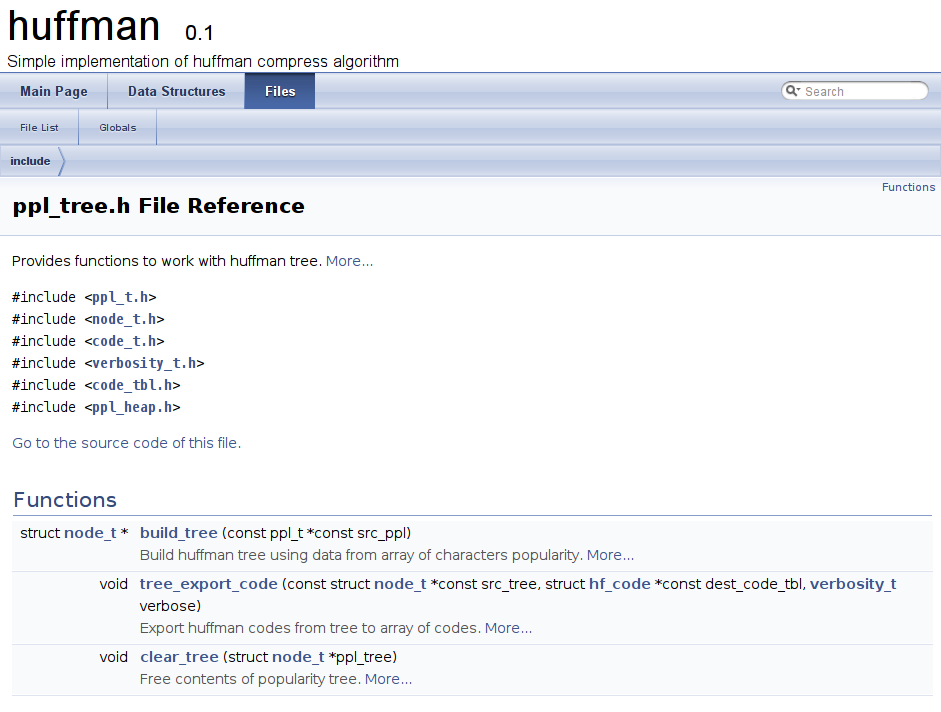
\includegraphics[width=150mm]{pic/documentation.png}
  \caption{Пример страницы документации}
  \label{pic:documentation}
\end{figure}
